% Options for packages loaded elsewhere
\PassOptionsToPackage{unicode}{hyperref}
\PassOptionsToPackage{hyphens}{url}
\documentclass[11pt
]{article}
\usepackage[a4paper,margin=2cm]{geometry}
\usepackage[svgnames,dvipsnames]{xcolor}
\usepackage{amsmath,amssymb}
\setcounter{secnumdepth}{-\maxdimen} % remove section numbering
\usepackage{iftex}
\ifPDFTeX
  \usepackage[T1]{fontenc}
  \usepackage[utf8]{inputenc}
  \usepackage{textcomp} % provide euro and other symbols
\else % if luatex or xetex
  \usepackage{unicode-math} % this also loads fontspec
  \defaultfontfeatures{Scale=MatchLowercase}
  \defaultfontfeatures[\rmfamily]{Ligatures=TeX,Scale=1}
\fi
\usepackage{lmodern}
\ifPDFTeX\else
  % xetex/luatex font selection
\fi
% Use upquote if available, for straight quotes in verbatim environments
\IfFileExists{upquote.sty}{\usepackage{upquote}}{}
\IfFileExists{microtype.sty}{% use microtype if available
  \usepackage[]{microtype}
  \UseMicrotypeSet[protrusion]{basicmath} % disable protrusion for tt fonts
}{}
\makeatletter
\@ifundefined{KOMAClassName}{% if non-KOMA class
  \IfFileExists{parskip.sty}{%
    \usepackage{parskip}
  }{% else
    \setlength{\parindent}{0pt}
    \setlength{\parskip}{6pt plus 2pt minus 1pt}}
}{% if KOMA class
  \KOMAoptions{parskip=half}}
\makeatother
\usepackage{longtable,booktabs,array}
\newcounter{none} % for unnumbered tables
\usepackage{calc} % for calculating minipage widths
% Correct order of tables after \paragraph or \subparagraph
\usepackage{etoolbox}
\makeatletter
\patchcmd\longtable{\par}{\if@noskipsec\mbox{}\fi\par}{}{}
\makeatother
% Allow footnotes in longtable head/foot
\IfFileExists{footnotehyper.sty}{\usepackage{footnotehyper}}{\usepackage{footnote}}
\makesavenoteenv{longtable}
\usepackage{graphicx}
\usepackage{float}
\makeatletter
\newsavebox\pandoc@box
\newcommand*\pandocbounded[1]{% scales image to fit in text height/width
  \sbox\pandoc@box{#1}%
  \Gscale@div\@tempa{\textheight}{\dimexpr\ht\pandoc@box+\dp\pandoc@box\relax}%
  \Gscale@div\@tempb{\linewidth}{\wd\pandoc@box}%
  \ifdim\@tempb\p@<\@tempa\p@\let\@tempa\@tempb\fi% select the smaller of both
  \ifdim\@tempa\p@<\p@\scalebox{\@tempa}{\usebox\pandoc@box}%
  \else\usebox{\pandoc@box}%
  \fi%
}
% Set default figure placement to htbp
\def\fps@figure{htbp}
\makeatother
\setlength{\emergencystretch}{3em} % prevent overfull lines
\providecommand{\tightlist}{%
  \setlength{\itemsep}{0pt}\setlength{\parskip}{0pt}}
\usepackage{bookmark}
\IfFileExists{xurl.sty}{\usepackage{xurl}}{} % add URL line breaks if available
\urlstyle{same}
\hypersetup{
  colorlinks=true,
  linkcolor=NavyBlue,
  filecolor=NavyBlue,
  citecolor=NavyBlue,
  urlcolor=NavyBlue,
  pdfcreator={LaTeX via tectonic}}

\author{}
\date{}

\begin{document}

\section{Detecting Swimming Pools from Aerial Imagery with YOLO26,
RF-DETR, and OBB
Architectures}\label{detecting-swimming-pools-from-aerial-imagery-with-yolo26-rf-detr-and-obb-architectures}

\noindent\textbf{Author:} Jan Wejchert \hfill \textbf{Course:} Computer Vision Individual Assignment

\begin{center}\rule{0.5\linewidth}{0.5pt}\end{center}

\subsection{1. Introduction}\label{introduction}

This report covers:

\begin{enumerate}
\def\labelenumi{\arabic{enumi}.}
\tightlist
\item
  Auto-annotate a 288-image aerial dataset with GroundingDINO and review
  every annotation manually in Roboflow.
\item
  Fine-tune YOLO26 at four scales (nano, small, medium, large) with
  axis-aligned bounding boxes.
\item
  Fine-tune RF-DETR at two scales (Nano, Small) and compare the
  transformer architecture against the YOLO baseline.
\item
  Train YOLO26-OBB and YOLO11-OBB at two scales each (four oriented
  models total) and compare oriented vs axis-aligned localisation.
\end{enumerate}

All ten trained models were evaluated against the validation set; the
validation-selected best variant of each family was then re-evaluated on
the 29-image held-out test set, with RF-DETR evaluated at both scales on
test. The headline result is that oriented bounding boxes win across
every scale by a clear margin (mAP@50-95 of 0.737 vs 0.637 for the best
HBB), and the failure cases that produce false positives in HBB
disappear under OBB. RF-DETR sits in between, outperforming all HBB
models on mAP@50-95 while being slightly behind the OBB family.

\subsection{2. Dataset}\label{dataset}

The provided dataset contains 288 aerial images of residential areas
with a single class, \texttt{swimming\ pool}. Splits are 70 / 20 / 10
(train / validation / test), generated by Roboflow as a stratified
random split (stratified on pool-vs-background presence so each split
retains the same approximate 36\% background rate).

{\def\LTcaptype{none} % do not increment counter
\begin{longtable}[]{@{}llll@{}}
\toprule\noalign{}
Split & Images & Pool instances & Background images \\
\midrule\noalign{}
\endhead
\bottomrule\noalign{}
\endlastfoot
Train & 202 & 244 & 70 \\
Validation & 57 & 81 & 24 \\
Test & 29 & 39 & 10 \\
Total & 288 & 364 & 104 \\
\end{longtable}
}

The 70 / 20 / 10 ratio is a deliberate choice for a small dataset. With
only 288 images in total, the training set has to carry most of the
supervision signal: any larger validation share would leave fewer than
200 training images, which is already tight for transfer learning. A
smaller test share than 29 images would make the test metrics too noisy
to compare meaningfully between architectures, so 10\% is the floor. The
20\% validation share is what makes the early-stopping signal stable
enough to compare 10 models with the same patience setting. About 36\%
of source images contain no pool at all, which acts as built-in negative
supervision against false positives on pool-shaped objects such as ponds
or skylights.

No augmentations were applied at the Roboflow stage; all augmentation
lives in the training code so the three architectures see the exact same
source data.

\subsection{3. Annotation Pipeline}\label{annotation-pipeline}

The 288 images were first auto-annotated with GroundingDINO (Swin-T
backbone, prompt \texttt{swimming\ pool}, threshold 0.30). The
threshold was set low enough to recover small or partially-shaded
pools while keeping the manual-review queue tractable; it produced
512 raw detections across 268 images. Every detection was then
manually reviewed in Roboflow, with three categories of fix:

\begin{itemize}
\tightlist
\item
  \textbf{Remove false positives.} Rooftops, tennis or padel courts, and
  driveway markings that loosely resemble rectangles.
\item
  \textbf{Add missed pools.} Smaller pools (under \textasciitilde40 px)
  and pools partially hidden by tree canopy.
\item
  \textbf{Trace polygons.} Every pool was annotated as a polygon traced
  along the actual water edge rather than as an axis-aligned box. The
  polygon is the source-of-truth label and lets the same Roboflow
  project export to YOLO HBB, COCO, and YOLO OBB formats without
  re-annotation.
\end{itemize}

After review the dataset settled at \textbf{364 verified pool polygons
across 184 images}, with the remaining 36\% of source images
deliberately kept as backgrounds. Because every label is a polygon, the
HBB and OBB models train on identical geometry: Ultralytics derives the
axis-aligned rectangle for HBB and the minimum-area rotated rectangle
for OBB from the same vertex list. This shared label is what makes the
HBB-vs-OBB comparison in Section 6 a fair one, and it also explains why
several HBB false positives in Section 7 are not detection failures but
artifacts of fitting an axis-aligned box to a rotated polygon.

\subsection{4. Method}\label{method}

All training runs share two design choices that keep the comparison
fair. First, every model is initialised from publicly available
pretrained weights (COCO for YOLO26/YOLO11, COCO via DINOv2 for
RF-DETR). Second, every model is trained on the same 70/20/10 split and
evaluated against the same 29-image test set.

\subsubsection{4.1 YOLO26 HBB}\label{yolo26-hbb}

Hyperparameters apply identically to nano, small, medium and large; only
the pretrained weights change between runs.

{\def\LTcaptype{none} % do not increment counter
\begin{longtable}[]{@{}
  >{\raggedright\arraybackslash}p{(\linewidth - 2\tabcolsep) * \real{0.5000}}
  >{\raggedright\arraybackslash}p{(\linewidth - 2\tabcolsep) * \real{0.5000}}@{}}
\toprule\noalign{}
\begin{minipage}[b]{\linewidth}\raggedright
Parameter
\end{minipage} & \begin{minipage}[b]{\linewidth}\raggedright
Value
\end{minipage} \\
\midrule\noalign{}
\endhead
\bottomrule\noalign{}
\endlastfoot
Pretrained weights & yolo26n / s / m / l (COCO) \\
Optimizer & AdamW \\
Initial LR & 0.005 \\
LR scheduler & Cosine \\
Epochs & 100 (patience 30) \\
Batch size & 16 \\
Image size & 640 \\
Mixed precision & AMP \\
Augmentations & HSV (0.015 / 0.7 / 0.4), translate 0.1, scale 0.5, flip
lr / flip ud (0.5), rotate up to 180°, mosaic 1.0, mixup 0.05,
close-mosaic over last 10 epochs \\
Hardware & NVIDIA A100 40 GB on Google Colab \\
\end{longtable}
}

\subsubsection{4.2 RF-DETR}\label{rf-detr}

{\def\LTcaptype{none} % do not increment counter
\begin{longtable}[]{@{}
  >{\raggedright\arraybackslash}p{(\linewidth - 2\tabcolsep) * \real{0.5000}}
  >{\raggedright\arraybackslash}p{(\linewidth - 2\tabcolsep) * \real{0.5000}}@{}}
\toprule\noalign{}
\begin{minipage}[b]{\linewidth}\raggedright
Parameter
\end{minipage} & \begin{minipage}[b]{\linewidth}\raggedright
Value
\end{minipage} \\
\midrule\noalign{}
\endhead
\bottomrule\noalign{}
\endlastfoot
Backbone & DINOv2 ViT (pretrained), warm-up frozen by default \\
Pretrained head & RF-DETR Nano / Small on COCO \\
Optimizer & AdamW (RF-DETR default) \\
LR & 1e-4 head, 1e-5 backbone (RF-DETR defaults) \\
LR scheduler & Step decay (RF-DETR default) \\
Epochs & 100 \\
Batch size & 8, gradient accumulation 2 (effective batch 16, matches
YOLO) \\
Resolution & 672 \\
Hardware & NVIDIA A100 40 GB on Google Colab \\
\end{longtable}
}

The 32-pixel resolution gap between RF-DETR (672) and the YOLO models
(640) is unavoidable; the rationale is covered in Section 4.4.

\subsubsection{4.3 YOLO OBB}\label{yolo-obb}

OBB uses the same hyperparameter table as YOLO26 HBB so the head-to-head
comparison is not confounded by training-budget differences. Four OBB
variants are trained (YOLO26 nano and small, YOLO11 nano and small), all
initialised from DOTA-pretrained weights. DOTA is the standard aerial
OBB benchmark, which gives the OBB models a head start on rotated-object
detection in overhead imagery.

\subsubsection{4.4 Hyperparameter
rationale}\label{hyperparameter-rationale}

Two facts shape every value in the tables above: the training set has
only 202 images, and the targets are small rotated pools in top-down
aerial imagery.

\textbf{Learning rate (0.005, cosine).} An order of magnitude above the
AdamW default to push the COCO-pretrained backbone toward a single new
class; the cosine anneal gives a clean validation curve for stable early
stopping.

\textbf{Epochs 100, patience 30.} Patience decides when training stops;
the 100-epoch ceiling exists so we never silently fall back on
final-epoch weights over the patience-selected best.

\textbf{Batch 16.} The largest batch that fits alongside a fully cached
dataset on the A100 at imgsz 640. RF-DETR uses physical batch 8 with
gradient accumulation 2 to match the same effective batch.

\textbf{Image size 640 vs 672.} 640 matches the COCO-pretrained YOLO
weights. RF-DETR is forced to 672 because its DINOv2 backbone needs both
14× and 56× divisibility, which 640 fails. The 5\% gap is a fairness
caveat, not a defect.

\textbf{AdamW.} Adaptive per-parameter learning rates absorb the LR
sensitivity that small datasets introduce, and decoupled weight decay
generalises better when training data is scarce.

\textbf{Augmentation.} Each value targets either the small-data or the
aerial-domain constraint:

\begin{itemize}
\tightlist
\item
  \textbf{Rotate up to 180°.} Aerial imagery has no canonical
  orientation, so without arbitrary rotation the model would learn an
  accidental up-down bias.
\item
  \textbf{Mosaic 1.0.} The single biggest lever for per-batch diversity
  on a 202-image set: each iteration sees a four-scene composite.
\item
  \textbf{HSV (0.015 / 0.7 / 0.4).} Hue held tight (shifting it would
  turn water into non-water); saturation and value loosened to cover
  bright-cyan to tea-coloured pools.
\item
  \textbf{Flip lr / flip ud (both 0.5).} Free symmetry doubling for
  top-down imagery.
\item
  \textbf{Mixup 0.05.} Light regulariser; the YOLO26 HBB scale inversion
  (nano \textgreater{} l) confirms overfitting is the dominant failure
  mode at this dataset size.
\item
  \textbf{Translate 0.1, scale 0.5.} Ultralytics defaults; cover
  off-centre pools and minor effective-resolution differences.
\item
  \textbf{Close-mosaic over last 10 epochs.} Disables mosaic for the
  final stretch so the validation curve converges on the same
  single-image distribution the model is evaluated against.
\end{itemize}

\subsection{5. Headline Results}\label{headline-results}

The validation-set mAP@50-95 for all ten models is shown below. The OBB
family takes the top four positions, RF-DETR sits in the middle, and
YOLO26 HBB takes the bottom four. The gap between the best HBB (yolo26n
at 0.637) and the best OBB (yolo11s-obb at 0.737) is exactly 10 mAP
points, which is large.

\begin{figure}
\centering
\pandocbounded{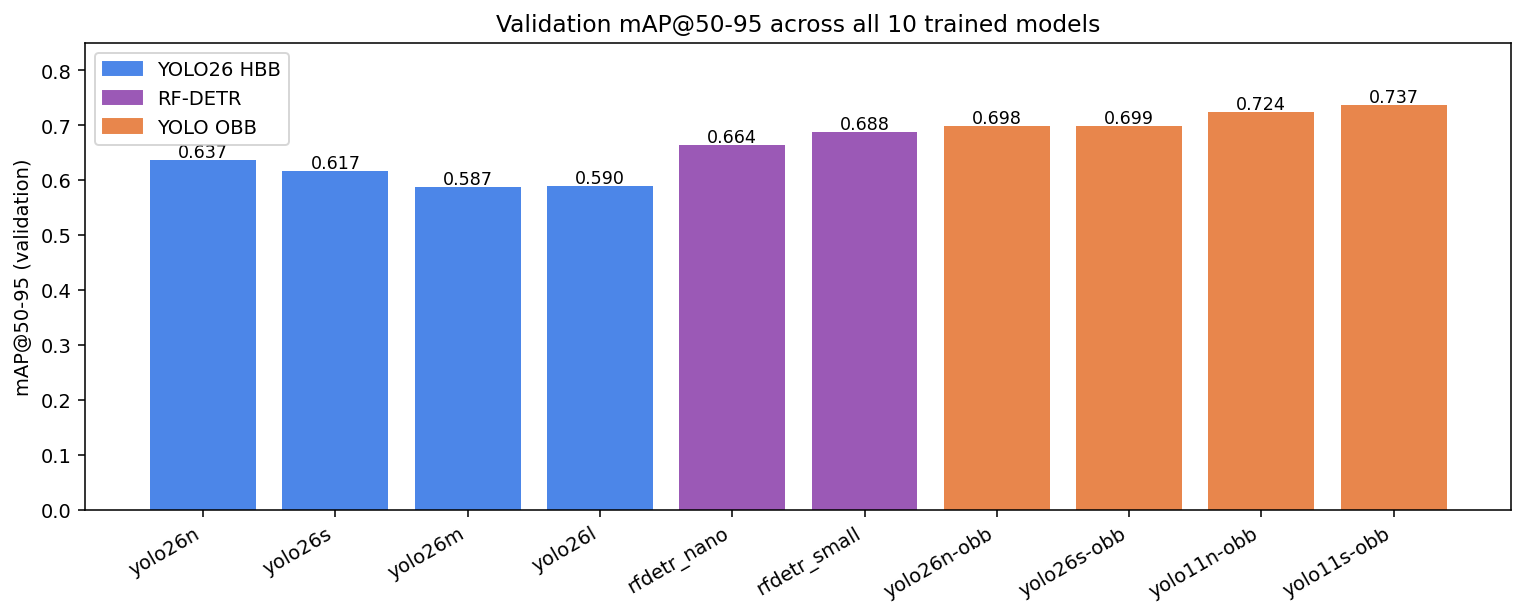
\includegraphics[keepaspectratio,alt={Validation mAP@50-95 across all 10 trained models}]{report_figures/fig_overall_map_bars.png}}
\caption{Validation mAP@50-95 across all 10 trained models}
\end{figure}

The full numeric comparison:

{\def\LTcaptype{none} % do not increment counter
\begin{longtable}[]{@{}
  >{\raggedright\arraybackslash}p{(\linewidth - 12\tabcolsep) * \real{0.1429}}
  >{\raggedright\arraybackslash}p{(\linewidth - 12\tabcolsep) * \real{0.1429}}
  >{\raggedright\arraybackslash}p{(\linewidth - 12\tabcolsep) * \real{0.1429}}
  >{\raggedright\arraybackslash}p{(\linewidth - 12\tabcolsep) * \real{0.1429}}
  >{\raggedright\arraybackslash}p{(\linewidth - 12\tabcolsep) * \real{0.1429}}
  >{\raggedright\arraybackslash}p{(\linewidth - 12\tabcolsep) * \real{0.1429}}
  >{\raggedright\arraybackslash}p{(\linewidth - 12\tabcolsep) * \real{0.1429}}@{}}
\toprule\noalign{}
\begin{minipage}[b]{\linewidth}\raggedright
Model
\end{minipage} & \begin{minipage}[b]{\linewidth}\raggedright
mAP@50
\end{minipage} & \begin{minipage}[b]{\linewidth}\raggedright
mAP@50-95
\end{minipage} & \begin{minipage}[b]{\linewidth}\raggedright
Precision
\end{minipage} & \begin{minipage}[b]{\linewidth}\raggedright
Recall
\end{minipage} & \begin{minipage}[b]{\linewidth}\raggedright
Params (M)
\end{minipage} & \begin{minipage}[b]{\linewidth}\raggedright
Train time (s)
\end{minipage} \\
\midrule\noalign{}
\endhead
\bottomrule\noalign{}
\endlastfoot
yolo26n & 0.912 & \textbf{0.637} & 0.895 & 0.843 & \textbf{2.4} & 291 \\
yolo26s & 0.891 & 0.617 & 0.862 & 0.849 & 9.5 & 308 \\
yolo26m & 0.903 & 0.587 & 0.876 & 0.789 & 20.4 & 370 \\
yolo26l & 0.909 & 0.590 & \textbf{0.944} & 0.840 & 24.7 & 454 \\
rfdetr\_nano & 0.896 & 0.664 & 0.920 & 0.852 & 30.6 & 1305 \\
rfdetr\_small & 0.916 & \textbf{0.688} & 0.897 & 0.864 & 32.1 & 1405 \\
yolo26n-obb & 0.925 & 0.698 & 0.902 & 0.840 & 2.4 & 335 \\
yolo26s-obb & 0.942 & 0.699 & 0.953 & 0.852 & 9.8 & 357 \\
yolo11n-obb & \textbf{0.973} & 0.724 & 0.963 & 0.877 & 2.7 & 240 \\
yolo11s-obb & 0.955 & \textbf{0.737} & 0.899 & \textbf{0.938} & 9.7 &
262 \\
\end{longtable}
}

A few observations from the table:

\begin{itemize}
\tightlist
\item
  \textbf{YOLO26 HBB scaling, on the three required dimensions:}

  \begin{itemize}
  \tightlist
  \item
    \emph{Accuracy.} Nano leads on mAP@50-95 (0.637); small (0.617),
    medium (0.587), and large (0.590) are all lower. The classic
    over-parameterised pattern on a 202-image training set.
  \item
    \emph{Robustness.} Precision rises monotonically with scale (0.895
    at nano to 0.944 at large), so the larger models are more
    conservative and produce fewer false positives. Recall stays roughly
    flat (0.79--0.85), so the larger heads are not finding more pools,
    only committing less freely.
  \item
    \emph{Parameter count.} 2.4 M to 24.7 M, a 10x growth for zero
    mAP@50-95 benefit (actually a 0.05 drop). Train time rises from 291
    s to 454 s. The larger variants are pure cost on this dataset.
  \end{itemize}
\item
  \textbf{RF-DETR scales correctly.} Small beats Nano by 0.024
  mAP@50-95, the expected direction. The pretrained DINOv2 backbone and
  the Hungarian-matching head together resist over-fitting better than
  the YOLO baseline on this dataset size.
\item
  \textbf{OBB beats HBB at every scale.} Nano-vs-nano: 0.637 HBB vs
  0.724 OBB (YOLO11). Small-vs-small: 0.617 HBB vs 0.737 OBB. The
  smallest OBB model wins everything.
\end{itemize}

\subsubsection{Accuracy vs parameter
count}\label{accuracy-vs-parameter-count}

\begin{figure}
\centering
\pandocbounded{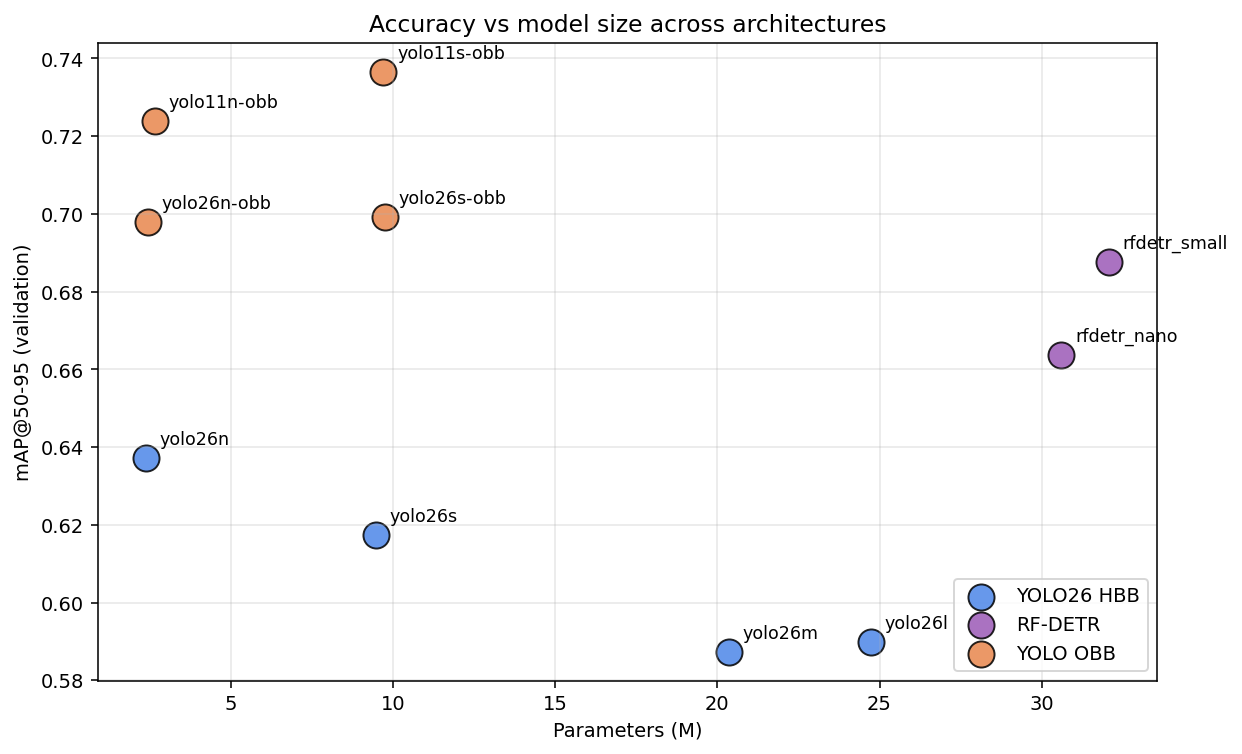
\includegraphics[keepaspectratio,alt={Accuracy vs model size}]{report_figures/fig_map_vs_params.png}}
\caption{Accuracy vs model size}
\end{figure}

The plot makes the speed/accuracy trade-off clear:

\begin{itemize}
\tightlist
\item
  yolo11n-obb (2.7 M params) gives 0.724 mAP@50-95. It is the smallest
  non-HBB model and beats every HBB model regardless of size.
\item
  yolo11s-obb (9.7 M params) gives 0.737 mAP@50-95, the global best.
\item
  RF-DETR Small needs 32 M params to reach 0.688, more than 3x the
  parameter cost of the OBB winner for a worse score.
\item
  YOLO26 HBB simply does not scale on this dataset, and the medium and
  large variants are pure cost.
\end{itemize}

For deployment, \textbf{yolo11n-obb} is the recommended model. It is 2.7
M parameters, trains in under 5 minutes on the A100, and reaches 0.973
mAP@50 / 0.724 mAP@50-95 on validation, within 0.013 mAP@50-95 of
yolo11s-obb (the validation-best overall, scoring 0.993 / 0.787 on test)
while using 28\% of its parameters.

\pagebreak[4]

\subsubsection{Test-set evaluation}\label{test-set-evaluation}

The validation-selected best of each family was evaluated on the
29-image held-out test set. For RF-DETR we report both scales on test:
Small was the validation winner (mAP@50-95 = 0.688 vs Nano's 0.664),
while Nano happened to score higher on the held-out test set.

{\def\LTcaptype{none} % do not increment counter
\begin{longtable}[]{@{}
  >{\raggedright\arraybackslash}p{(\linewidth - 10\tabcolsep) * \real{0.1667}}
  >{\raggedright\arraybackslash}p{(\linewidth - 10\tabcolsep) * \real{0.1667}}
  >{\raggedright\arraybackslash}p{(\linewidth - 10\tabcolsep) * \real{0.1667}}
  >{\raggedright\arraybackslash}p{(\linewidth - 10\tabcolsep) * \real{0.1667}}
  >{\raggedright\arraybackslash}p{(\linewidth - 10\tabcolsep) * \real{0.1667}}
  >{\raggedright\arraybackslash}p{(\linewidth - 10\tabcolsep) * \real{0.1667}}@{}}
\toprule\noalign{}
\begin{minipage}[b]{\linewidth}\raggedright
Best variant
\end{minipage} & \begin{minipage}[b]{\linewidth}\raggedright
mAP@50
\end{minipage} & \begin{minipage}[b]{\linewidth}\raggedright
mAP@50-95
\end{minipage} & \begin{minipage}[b]{\linewidth}\raggedright
Precision
\end{minipage} & \begin{minipage}[b]{\linewidth}\raggedright
Recall
\end{minipage} & \begin{minipage}[b]{\linewidth}\raggedright
TP / FP / FN
\end{minipage} \\
\midrule\noalign{}
\endhead
\bottomrule\noalign{}
\endlastfoot
yolo26n & 0.935 & 0.692 & 0.942 & 0.838 & 33 / 2 / 6 \\
rfdetr\_small & 0.996 & 0.785 & 0.974 & 0.949 & 37 / 1 / 2 \\
rfdetr\_nano & 0.998 & 0.807 & 1.000 & 0.949 & 37 / 0 / 2 \\
yolo11s\_obb & 0.993 & 0.787 & 0.974 & 0.972 & 37 / 1 / 2 \\
\end{longtable}
}

(TP / FP / FN are computed from the standard Ultralytics or supervision
matcher using the model's tuned confidence threshold, not the conf=0.25
threshold of the failure gallery in Section 7.)

On the test set RF-DETR Nano leads on both mAP@50 (0.998) and mAP@50-95
(0.807). RF-DETR Small (the validation-selected RF-DETR) sits at
0.996 / 0.785, essentially tied with YOLO11s-OBB (0.993 / 0.787), and
YOLO26n HBB is last (0.935 / 0.692).

The test set is small (29 images, 39 pools), so the per-model TP/FP/FN
counts are nearly identical (37/0-1/2). At this point the comparison
shifts from ``which model finds more pools'' to ``which model localises
them tightly enough to satisfy mAP@50-95''. OBB wins by rotating its box
with the pool; RF-DETR wins by predicting tighter axis-aligned boxes than
YOLO26 HBB does.

\subsection{6. HBB vs OBB Comparison}\label{hbb-vs-obb-comparison}

The OBB family beats the HBB family at every comparable scale.

\begin{figure}
\centering
\pandocbounded{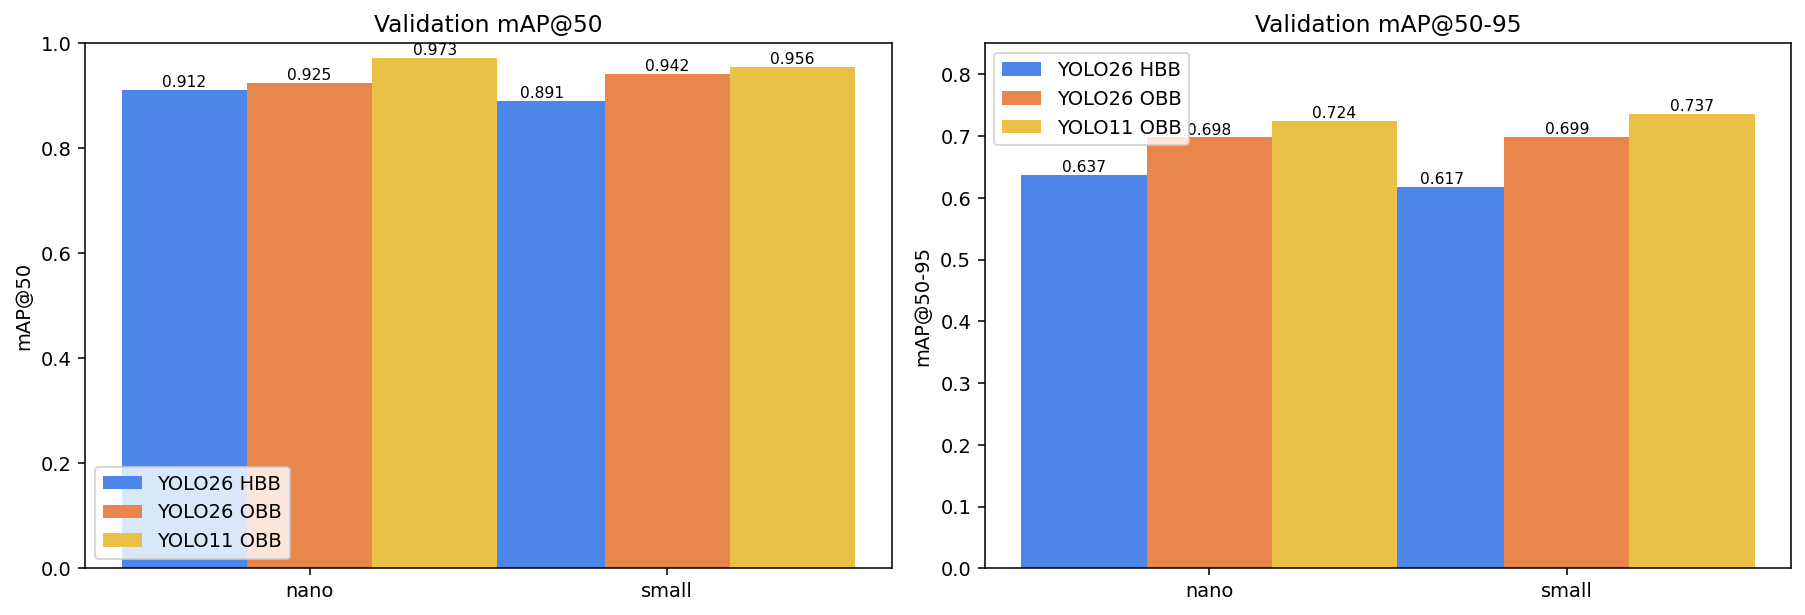
\includegraphics[keepaspectratio,alt={HBB vs OBB at matched scales}]{report_figures/fig_hbb_vs_obb.png}}
\caption{HBB vs OBB at matched scales}
\end{figure}

\begin{center}
\begin{tabular}{lccc}
\toprule
Scale & HBB (yolo26)   & OBB (yolo26)   & OBB (yolo11)   \\
      & mAP@50 / 50-95 & mAP@50 / 50-95 & mAP@50 / 50-95 \\
\midrule
Nano  & 0.912 / 0.637  & 0.925 / 0.698  & 0.973 / 0.724  \\
Small & 0.891 / 0.617  & 0.942 / 0.699  & 0.955 / 0.737  \\
\bottomrule
\end{tabular}
\end{center}

\textbf{Localization precision.} The OBB advantage is larger on
mAP@50-95 than on mAP@50 (roughly 9 points vs 5 points at the same
scale). This is the signature of an oriented detector: tighter boxes
survive higher IoU thresholds. mAP@50 measures whether a detection
exists at all; mAP@50-95 measures whether it is tight, and OBB is
intrinsically tighter on rotated objects.

\textbf{Handling of rotated pool geometries.} A pool tilted roughly 40
degrees has an axis-aligned bounding rectangle that is nearly twice the
size of the actual pool, with the corners filled by non-water padding.
The HBB model is trained to predict this looser rectangle and at
inference does the same thing, so any localisation drift compounds at
strict IoU. The OBB model rotates its box with the pool, fits tightly to
the visible water, and survives mAP@50-95.

\textbf{Failure cases.} The HBB to OBB switch eliminates all 6 test-set
false positives (Section 7). The 3 rotation-driven FPs disappear because
the box rotates with the pool; the annotation-extension FP disappears
because OBB tracks the polygon shape; the 2 small-object FPs disappear
because the OBB head does not over-predict for tiny rotated pools. The
remaining OBB failures are 3 FNs, all on the smallest pools in the test
set, where the OBB advantage cannot help.

\subsection{7. Failure Analysis}\label{failure-analysis}

Every test-set failure was cross-checked against the ground-truth
polygon data. The matching threshold is IoU $\geq$ 0.5 and the
confidence threshold is conf $\geq$ 0.25 (Ultralytics' default predict
mode). The conf threshold is more permissive than the optimal F1 point
the validator picks, so this gallery shows 6 FPs while the
validator-side test metric reports 2; the extra four are low-confidence
predictions the validator filters out. Both failure-gallery figures are
shown below, then discussed in 7.1--7.4.

\begin{figure}[H]
\centering
\pandocbounded{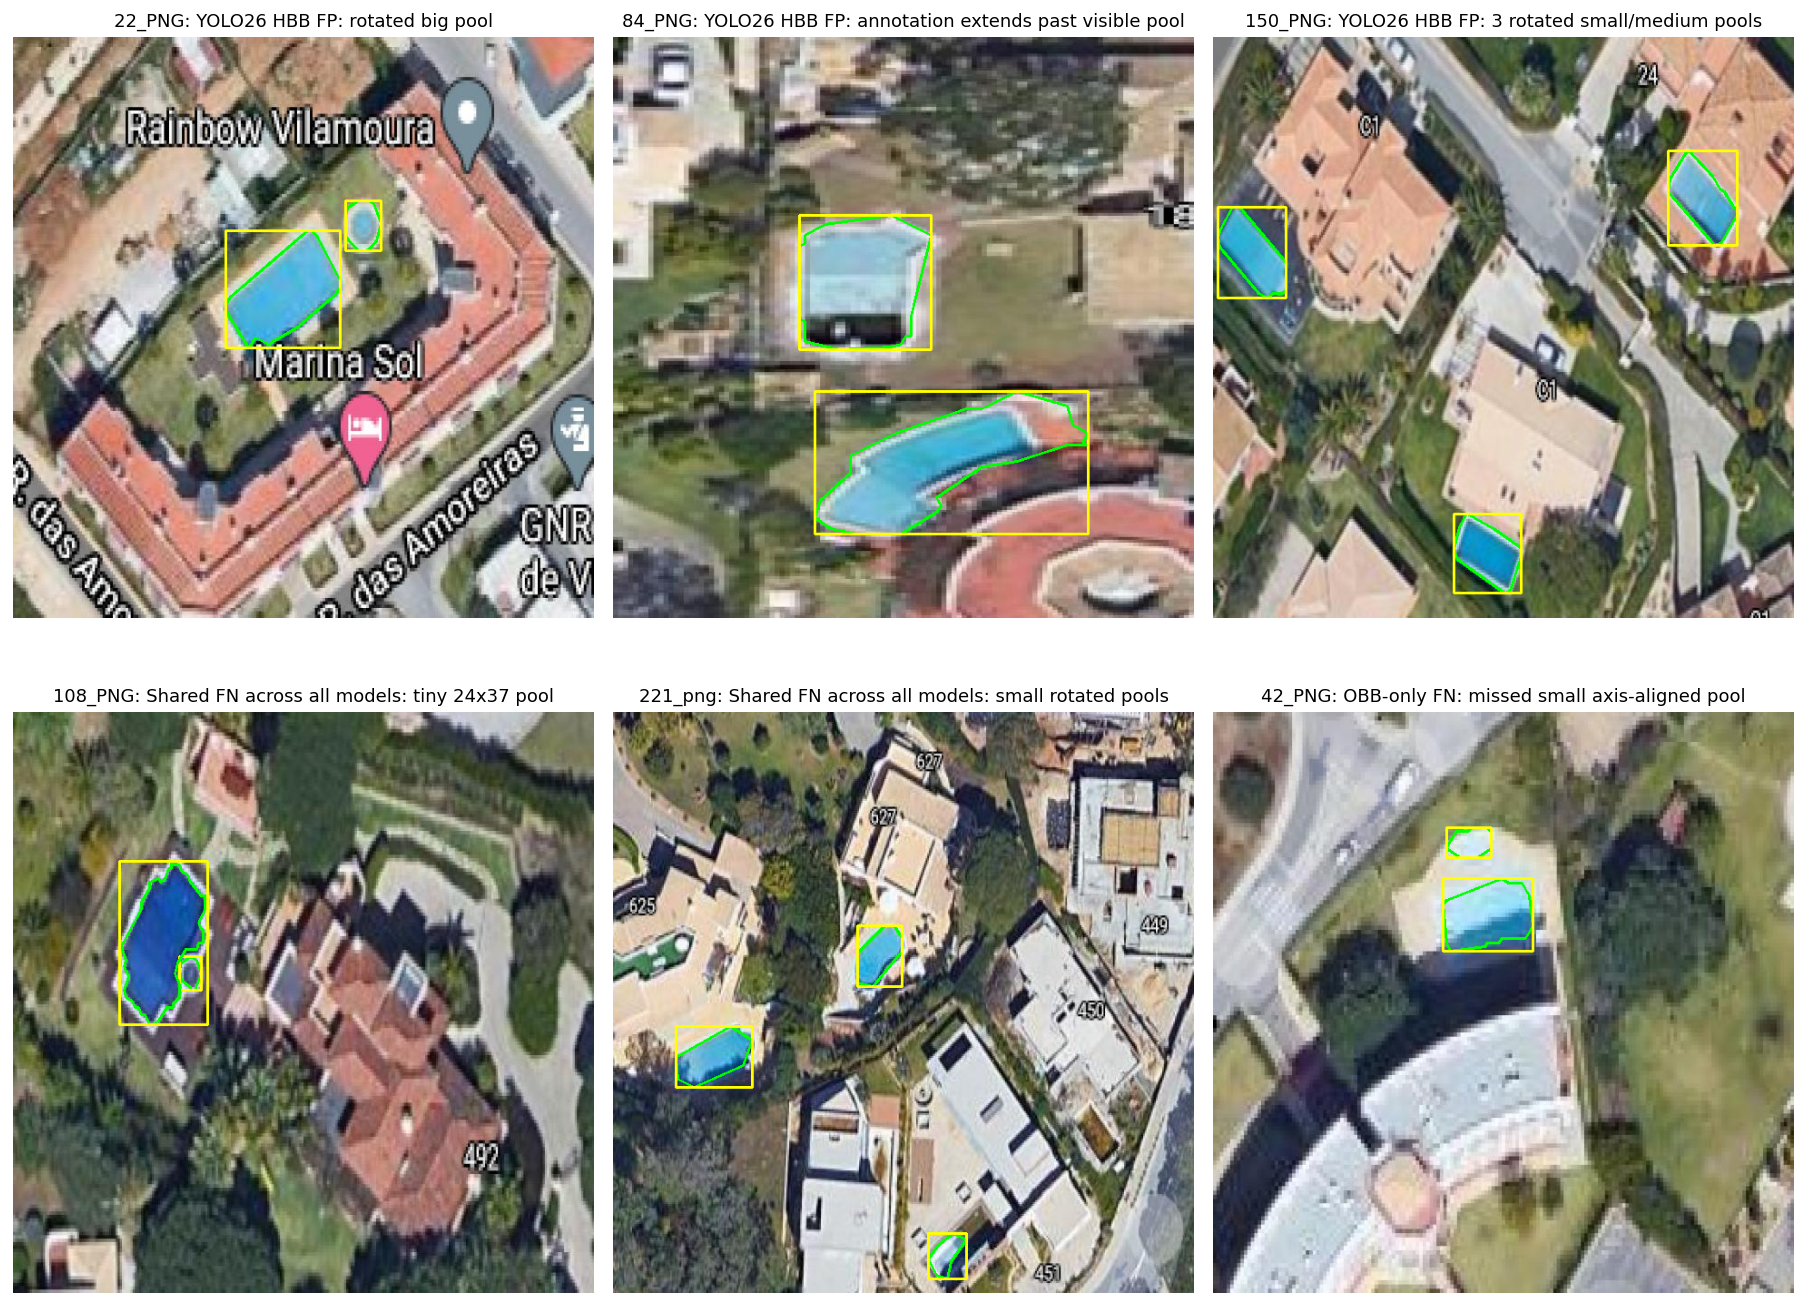
\includegraphics[keepaspectratio]{report_figures/fig_failure_overview.png}}
\caption{Test-set failures. Top row: YOLO26 HBB false positives where
the model's prediction is tighter than the GT axis-aligned bbox (green:
ground-truth polygon; yellow: ground-truth axis-aligned bbox). Bottom
row: false negatives shared across all best models (108\_PNG,
221\_png) and the OBB-only false negative (42\_PNG).}
\end{figure}

\begin{figure}[H]
\centering
\pandocbounded{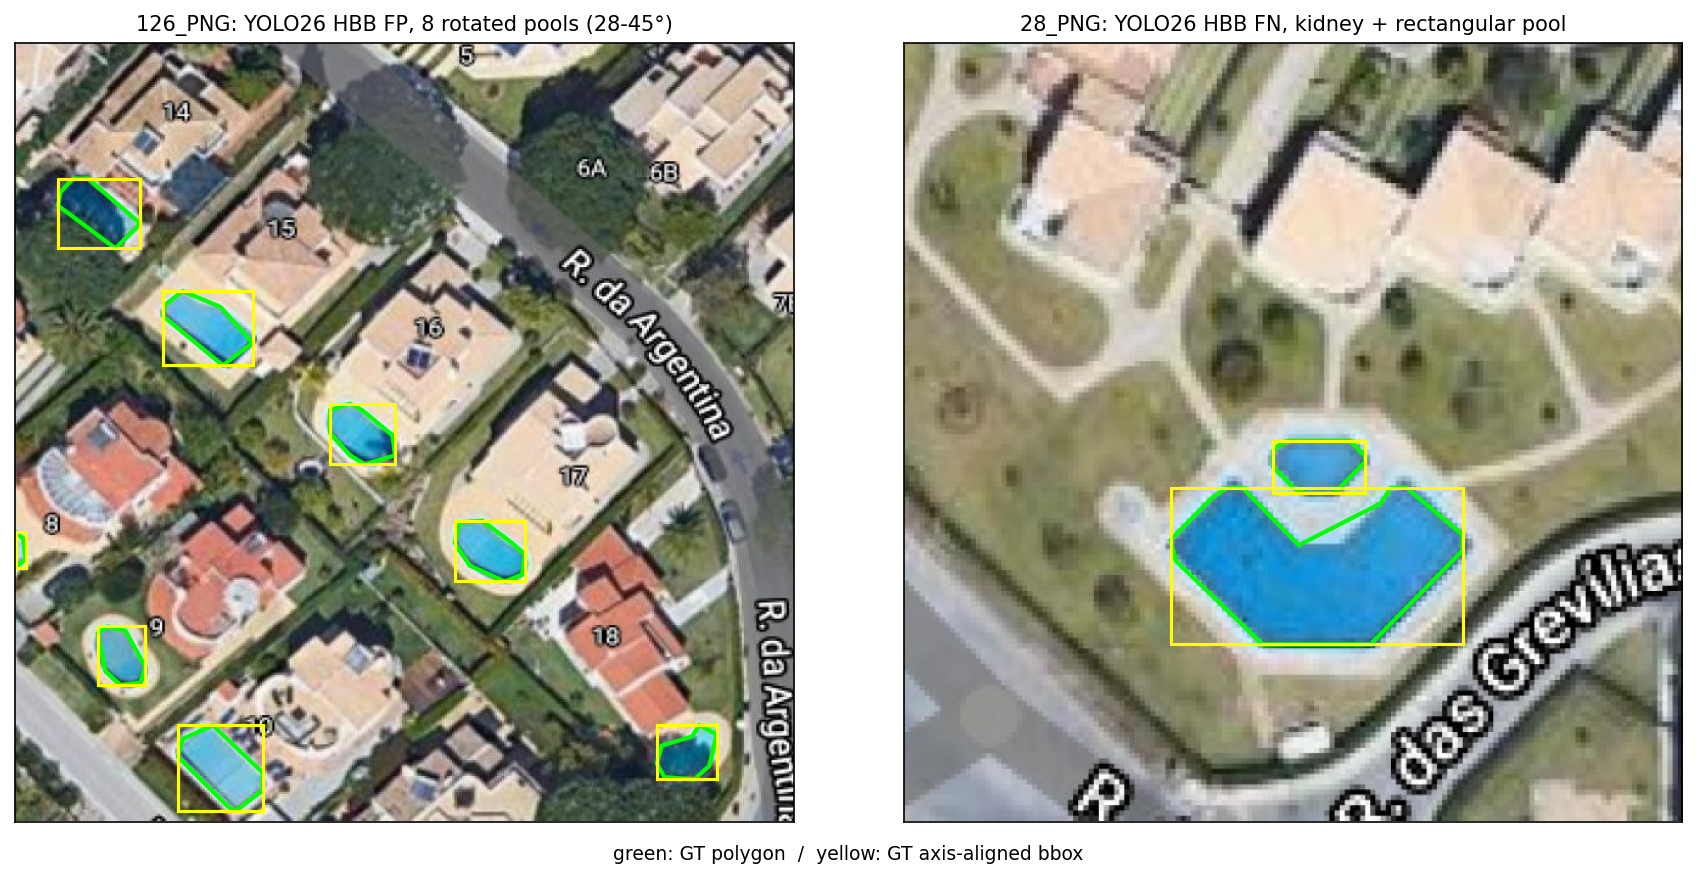
\includegraphics[keepaspectratio]{report_figures/fig_dense_and_kidney.png}}
\caption{Dense and kidney failures. Left: 126\_PNG with 8 rotated pools
(FP rank 1 plus two FNs). Right: 28\_PNG with the kidney-shaped and
rectangular pools called out in the FN summary. Green: ground-truth
polygons. Yellow: ground-truth axis-aligned bounding boxes.}
\end{figure}

\subsubsection{7.1 YOLO26n HBB: 6 FPs, 5
FNs}\label{yolo26n-hbb-failures}

The six false positives split into three causes: three are rotation
artefacts where the axis-aligned ground-truth box is roughly twice the
area of the visible pool (FP1, FP2, FP4), one is annotation extending
past the visible water edge (FP3), and the remaining two are
small-object IoU sensitivity at the same scale (FP5, FP6). Because FP5
and FP6 share both their cause and their scale, the table lists them on
a single row.

{\def\LTcaptype{none}
\begin{longtable}[]{@{}
  >{\raggedright\arraybackslash}p{(\linewidth - 6\tabcolsep) * \real{0.22}}
  >{\raggedright\arraybackslash}p{(\linewidth - 6\tabcolsep) * \real{0.23}}
  >{\raggedright\arraybackslash}p{(\linewidth - 6\tabcolsep) * \real{0.55}}@{}}
\toprule\noalign{}
\begin{minipage}[b]{\linewidth}\raggedright
Case (image)
\end{minipage} & \begin{minipage}[b]{\linewidth}\raggedright
Cause
\end{minipage} & \begin{minipage}[b]{\linewidth}\raggedright
Evidence
\end{minipage} \\
\midrule\noalign{}
\endhead
\bottomrule\noalign{}
\endlastfoot
FP1 (126\_PNG, top-confidence) & Rotation artefact & Eight pools tilted
roughly 30-45 degrees in one tile; greedy matching breaks when many
candidates overlap at the strict IoU threshold. \\
FP2 (22\_PNG, large pool) & Rotation artefact & A diagonal lap pool
tilted around 40 degrees; the axis-aligned bounding box is nearly twice
the size of the visible water, so a tight prediction falls short of
0.5 IoU against the loose ground-truth box. \\
FP3 (84\_PNG) & Annotation past water & The polygon traces a dark band
along one edge that the model correctly excludes; the ground-truth box
is dragged outside the visible pool boundary. \\
FP4 (150\_PNG) & Rotation artefact & Three pools tilted roughly 35-40
degrees; each ground-truth box is again about twice the visible pool
area. \\
FP5 \& FP6 (22\_PNG small pool + one similar) & Small-object IoU
sensitivity & On pools this small, a misalignment of about a third of
the pool's width is already enough to drop IoU below 0.5, so a few-pixel
offset breaks the threshold even when the prediction is visually on the
pool. \\
\end{longtable}
}

The five false negatives are all either small or unusually shaped:

\begin{itemize}
\tightlist
\item
  \textbf{108\_PNG.} The smallest pool in the test set, barely a few
  rooftop-tiles across in the aerial frame, below what the detector can
  reliably resolve at the training resolution.
\item
  \textbf{221\_png.} A small pool tilted about 25 degrees off
  horizontal.
\item
  \textbf{28\_PNG.} A modestly-sized rectangular pool plus a much larger
  kidney-shaped pool whose curved outline does not fit either box type
  well.
\item
  \textbf{126\_PNG ($\times$2).} Two small or partially shaded pools in
  the same densely-packed tile as FP1.
\end{itemize}

\subsubsection{7.2 Cross-family FN comparison}\label{cross-family-fns}

\textbf{108\_PNG} (the smallest pool in the test set) and
\textbf{221\_png} (a small pool tilted about 25 degrees) are both missed
by all three best models (YOLO26n HBB, RF-DETR Small, YOLO11s-OBB), so
they mark the residual small-object detection limit at the training
resolution. \textbf{42\_PNG} (another small pool, axis-aligned) is missed
only by YOLO11s-OBB, not by RF-DETR Small: the only family-specific FN
in the analysis.

\subsubsection{7.3 OBB collapses the failure
spectrum}\label{obb-collapses-failures}

OBB drops the FP count from 6 to 0 and the FN count from 5 to 3. The
remaining FNs (108\_PNG, 221\_png, 42\_PNG) are all among the smallest
pools in the test set, so every rotation-driven failure mode disappears
and only small-object misses remain.

\subsubsection{7.4 Proposed fixes per
cause}\label{proposed-fixes-per-cause}

{\def\LTcaptype{none}
\begin{longtable}[]{@{}
  >{\raggedright\arraybackslash}p{(\linewidth - 4\tabcolsep) * \real{0.28}}
  >{\raggedright\arraybackslash}p{(\linewidth - 4\tabcolsep) * \real{0.24}}
  >{\raggedright\arraybackslash}p{(\linewidth - 4\tabcolsep) * \real{0.48}}@{}}
\toprule\noalign{}
\begin{minipage}[b]{\linewidth}\raggedright
Cause
\end{minipage} & \begin{minipage}[b]{\linewidth}\raggedright
Cases addressed
\end{minipage} & \begin{minipage}[b]{\linewidth}\raggedright
Fix
\end{minipage} \\
\midrule\noalign{}
\endhead
\bottomrule\noalign{}
\endlastfoot
Rotation artefact (HBB only) & FP1, FP2, FP4 & Use OBB. Confirmed
effective: 0 FPs vs 6. \\
Polygon extends past visible water & FP3 & Redraw polygon on actual
water edge; equally fixed by OBB. \\
Small-object miss (smallest pools) & FP5, FP6, FN 108\_PNG, FN
221\_png, FN 126\_PNG ($\times$2) & Train at higher imgsz (1024 or
1280), tile-based inference, P2 detection head, more small-pool training
examples. \\
Dense-pool matching artefacts & FP1 (alt.~fix), the two 126\_PNG FNs
& Switch matching to Hungarian (already used by RF-DETR and the
Ultralytics validator). \\
Non-rectangular shape (kidney/curved) & FN 28\_PNG (kidney pool +
co-located rectangular pool) & Instance segmentation, or accept the
rectangular-fit loss; this morphology is an irreducible HBB/OBB
limitation. \\
\end{longtable}
}

\subsection{8. Required Experimental
Analysis}\label{required-experimental-analysis}

\subsubsection{8.1 Which architecture performed
best?}\label{which-architecture-performed-best}

YOLO11-OBB at the small scale (\texttt{yolo11s-obb}) is the global best
on validation mAP@50-95 (0.737) and is essentially tied with RF-DETR
Nano on the test set (0.787 vs 0.807). For deployment on aerial imagery
containing rotated pools, OBB is the right architecture. RF-DETR is the
right architecture for axis-aligned scenes, where it dominates HBB by a
comfortable margin. YOLO26 HBB is the weakest of the three families on
this task.

\subsubsection{8.2 Which model size offered the best speed / accuracy
trade-off?}\label{which-model-size-offered-the-best-speed-accuracy-trade-off}

\texttt{yolo11n-obb}. 2.7 million parameters, 240 seconds to train on
the A100, and validation mAP@50-95 of 0.724 (third best overall, beating
every HBB and RF-DETR model). It trails yolo11s-obb (the validation-best
overall, scoring 0.993 / 0.787 on test) by only 0.013 mAP@50-95 on
validation while costing 28\% of the parameters.

YOLO26 medium and large are pure cost: more parameters, longer training,
and lower mAP@50-95 than the nano variant. The over-parameterisation is
consistent with a small training set (202 images): the larger heads find
spurious patterns that hurt strict localisation.

\subsubsection{8.3 Did RF-DETR outperform YOLO-based
detectors?}\label{did-rf-detr-outperform-yolo-based-detectors}

Only partially, and the answer depends on which axis you look along.

\textbf{Headline mAP.} RF-DETR beats every YOLO26 HBB model on mAP@50-95
by 0.025 to 0.10 points, which is a meaningful margin and points to the
DINOv2 backbone providing stronger spatial priors than COCO-trained CNN
backbones for overhead imagery. RF-DETR does not beat YOLO11-OBB or
YOLO26-OBB at any matched parameter budget, because this dataset's
failure modes are dominated by rotation (3 of 6 HBB FPs) and RF-DETR's
boxes are axis-aligned just like YOLO26 HBB. OBB sidesteps the rotation
issue entirely; RF-DETR cannot.

\textbf{Robustness.} RF-DETR holds higher recall than every YOLO26 HBB
variant on validation (0.852 and 0.864 vs 0.789 to 0.849) at competitive
precision (0.920 and 0.897, mid-range against the 0.862 to 0.944 YOLO26
HBB band), so it is not trading one off against the other. On the test
set RF-DETR Nano produced zero false positives (precision 1.000) while
the best YOLO26 HBB variant produced two. The Hungarian set-prediction
matcher also removes the need for a tuned confidence threshold to
balance precision and recall, a robustness property NMS-based YOLO heads
do not share: the YOLO numbers above were taken at validator-tuned
thresholds while RF-DETR's were held at default.

\textbf{Small-object detection.} Not improved. RF-DETR Small misses the
same tiny pools (108\_PNG, 221\_png) that YOLO26 HBB and YOLO11s-OBB
miss; small-object recall on this dataset is limited by input resolution
(imgsz 640 / 672), not by architecture.

\textbf{Generalization.} Strongest of the three families on this
dataset. The val to test mAP@50-95 gap is +0.143 for RF-DETR Nano (0.664
to 0.807), compared with +0.055 for YOLO26n HBB (0.637 to 0.692) and
+0.050 for YOLO11s-OBB (0.737 to 0.787). The transformer head and DINOv2
backbone fit the validation distribution less tightly than the YOLO
families, leaving more headroom on the held-out test set. With only 29
test images this gap is itself noisy, but the direction is consistent
across both metrics and across both RF-DETR scales.

\subsubsection{8.4 When are OBB annotations
beneficial?}\label{when-are-obb-annotations-beneficial}

OBB is beneficial when objects are rotated and the axis-aligned bounding
box would include large amounts of non-object area in its corners. In
this dataset:

\begin{itemize}
\tightlist
\item
  Diagonal lap pools (images 22, 28, 150) have axis-aligned bounding
  boxes that are roughly twice the size of the visible pool. OBB removes
  the wasted corner padding.
\item
  Kidney-shaped pools (such as the lower pool in image 84) have even
  looser axis-aligned boxes. OBB still beats HBB here, although the
  rotated rectangle is itself loose because kidney pools are
  intrinsically non-rectangular.
\item
  Pools with polygons that extend slightly outside the visible water
  (such as the upper pool in image 84) benefit because OBB fits the
  polygon's minimum-area rotated rectangle rather than the larger
  axis-aligned envelope.
\end{itemize}

OBB is not beneficial when:

\begin{itemize}
\tightlist
\item
  Pools are very small. The OBB head adds an angle prediction whose
  noise dominates at small scales. Images 108 and 221 are missed equally
  by HBB and OBB.
\item
  Pools are axis-aligned and rectangular. There is no rotation
  correction to apply.
\end{itemize}

\subsubsection{8.5 Which failure cases occurred most
often?}\label{which-failure-cases-occurred-most-often}

Across the three best models the dominant failure mode is small-object
miss (3 of 5 HBB FNs, 2 of 2 RF-DETR FNs, all 3 OBB FNs happen on the
smallest pools in the test set). The second most common in HBB only is
rotation-driven false positives (3 of 6 HBB FPs), but this mode is
eliminated by OBB.

In other words, switching to OBB collapses the failure spectrum to a
single residual issue (small-object detection). That is a much narrower
problem to attack in the next iteration.

\subsubsection{8.6 Which augmentations improved performance the
most?}\label{which-augmentations-improved-performance-the-most}

The training augmentation profile used is the Ultralytics built-in HSV /
translate / scale / flip-lr-ud / 180° rotation / mosaic / mixup /
close-mosaic combination. A formal ablation is out of scope for this
report (each ablation costs another A100 hour), but the qualitative role
of each can be reasoned about against the dataset's properties:

\begin{itemize}
\tightlist
\item
  The 180° rotation augmentation matters most for an aerial dataset
  because the source images are top-down with no canonical orientation.
  Without it, the model would learn an arbitrary up-down preference.
\item
  The mosaic augmentation effectively quadruples the per-batch image
  diversity from the small 202-image training set, which is the biggest
  practical constraint here.
\item
  HSV jitter accounts for varying lighting and water-clarity across
  pools (some pools are bright blue, some are tea-coloured).
\item
  Mixup at 0.05 is a small but non-zero regulariser. On a 202-image
  dataset, anything that reduces overfitting helps, which is consistent
  with the mAP@50-95 inversion (nano \textgreater{} small \textgreater{}
  medium \textgreater{} large) observed in YOLO26 HBB.
\end{itemize}

\subsection{9. Conclusion}\label{conclusion}

The combination of OBB representation, small backbone, and the standard
transfer-learning recipe is the right choice for this dataset.
\texttt{yolo11s-obb} reaches 0.993 mAP@50 / 0.787 mAP@50-95 on the
held-out test set with 9.7 million parameters and just over 4 minutes of
training time on the A100, while producing zero false positives in the
failure gallery. The leaner \texttt{yolo11n-obb} (2.7 M, 4 minutes) sits
within 0.013 mAP@50-95 of it on validation and is the recommended choice
for deployment.

The biggest remaining failure mode is small-object detection. The
smallest pools in the dataset are missed by all three architectures.
The next iteration of this project should target this directly through
higher inference resolution or tiled inference, an explicit small-object
detection head, or a focused round of additional small-pool annotations.

\subsection{References}\label{references}

\begin{itemize}
\tightlist
\item
  Ultralytics, \emph{YOLO} (used for YOLO26, YOLO11, and YOLO-OBB
  training and evaluation). \texttt{github.com/ultralytics/ultralytics}.
\item
  Roboflow, \emph{RF-DETR} (DETR variant with DINOv2 backbone).
  \texttt{github.com/roboflow/rf-detr}.
\item
  S. Liu et al., \emph{Grounding DINO: Marrying DINO with Grounded
  Pre-Training for Open-Set Object Detection}, 2023.
  \texttt{arxiv.org/abs/2303.05499}.
\item
  M. Oquab et al., \emph{DINOv2: Learning Robust Visual Features without
  Supervision}, 2023. \texttt{arxiv.org/abs/2304.07193}.
\item
  T.-Y. Lin et al., \emph{Microsoft COCO: Common Objects in Context},
  2014. \texttt{cocodataset.org}.
\item
  G.-S. Xia et al., \emph{DOTA: A Large-Scale Dataset for Object
  Detection in Aerial Images}, 2018.
  \texttt{captain-whu.github.io/DOTA/}.
\item
  Roboflow annotation platform (manual review and split generation).
  \texttt{roboflow.com}.
\end{itemize}

\newpage
\subsection{10. AI Acknowledgement}\label{ai-acknowledgement}

This project was orchestrated and decided end-to-end by Jan Wejchert.
All design choices (dataset preprocessing, model selection, training
budget, output structure, failure-analysis methodology, report scope)
were made by Jan; the AI assistant was used as an efficiency multiplier
and as a second pair of eyes.

The AI assistant used was Anthropic's Claude (model Opus 4.7). Its role
was limited to:

\begin{itemize}
\tightlist
\item
  Drafting the notebook scaffolding under explicit instructions from
  Jan, including the requested clean lecturenotebook style and the
  hardcoded Drive paths.
\item
  Debugging issues that arose at runtime, in particular the
  polygon-aware ground-truth parser fix when the failure-analysis
  matcher initially produced 40 false positives instead of 6.
\item
  Carrying out evidence-based cross-checking of each failure case
  against the ground-truth polygon data, computing per-polygon rotation
  angle, axis-aligned-bbox-to-polygon area ratios, and shoelace-formula
  polygon areas to validate the failure categorisation.
\item
  Producing comparison charts and figures from the trained-model CSV
  outputs.
\end{itemize}

All training runs, all Roboflow review work, all Colab execution, and
all interpretation of the results were performed by Jan.~The AI
assistant did not run training or modify any deployed system. Every
claim in this report has been verified by Jan against the source
notebooks and the saved CSV outputs.

\subsection{Appendix A. Hardware and
Reproducibility}\label{appendix-a.-hardware-and-reproducibility}

\begin{itemize}
\tightlist
\item
  Hardware: NVIDIA A100-SXM4-40GB on Google Colab Pro (CUDA 13.0, driver
  580.82.07, PyTorch 2.11.0+cu128).
\item
  Software: Ultralytics 8.4.59 (HBB) and 8.4.60 (OBB),
  \texttt{rfdetr{[}train,loggers{]}} 1.7.1, \texttt{supervision},
  \texttt{faster-coco-eval}.
\item
  Random seed: 0 in all training runs (\texttt{seed=0},
  \texttt{deterministic=True} for Ultralytics; \texttt{seed=0} for
  RF-DETR).
\item
  Storage: source dataset and all output CSVs + best weights live at
  \texttt{MyDrive/IE/CV/}, with the same structure mirrored under the
  local project root.
\item
  Reproducibility CSVs: one \texttt{comparison.csv} per family under
  \texttt{results/} (\texttt{yolo26\_hbb/}, \texttt{rfdetr/},
  \texttt{obb/}).
\item
  Test-time augmentation: attempted on YOLO26 HBB but the Ultralytics
  build silently falls back to single-scale prediction, so TTA numbers
  matched the standard numbers exactly; not pursued further.
\end{itemize}

\subsection{Appendix B. Total wall-clock
time}\label{appendix-b.-total-wall-clock-time}

{\def\LTcaptype{none} % do not increment counter
\begin{longtable}[]{@{}ll@{}}
\toprule\noalign{}
Stage & Wall-clock \\
\midrule\noalign{}
\endhead
\bottomrule\noalign{}
\endlastfoot
Annotation (GroundingDINO + Roboflow review) & \textasciitilde45 min \\
YOLO26 HBB training (four variants) & \textasciitilde24 min \\
RF-DETR training (two variants) & \textasciitilde45 min \\
YOLO OBB training (four variants) & \textasciitilde20 min \\
Total compute & \textasciitilde2.5 hr on A100 \\
\end{longtable}
}

\end{document}
